\epigraph{To iterate is human, to recurse divine.}{L. Peter Deutsch}
\epigraph{To understand recursion, you must first understand recursion.}{Anon. ?}

\minitoc

In this chapter we show how to use recursive functions and C structs to sort data into a binary tree \cite{friend1956sorting,burge1958sorting,windley1960trees,walker1972hybrid} for fast retrieval of data proximal to query values. We introduce an important generalization of the binary tree called the quadtree that enables efficient retrieval of bi-variate (two-dimensional) data. We then describe how to use the quadtree data structure to find the nearest neighbor in a given set of two-dimensional data points a query point. The \href{https://en.wikipedia.org/wiki/Quadtree}{quadtree} algorithm was introduced in 1974 by Finkel and Benteley \cite{finkel1974quad,bentley1975multidimensional} as a two-dimensional generalization of the well known binary tree data structure used for storing one-dimensional data in a way that facilitates fast retrieval. 

The binary tree and quadtree both rely on recursively traversing a hierarchical tree data structure. In the following sections we first recall recursive functions before introducing an implementation of a binary tree followed by the quadtree data structure. We cap this off with a fast algorithm for locating the nearest data point in a quadtree to a query point.

\section{Recursion}
In this chapter we will use recursive functions, i.e. functions that call themselves. This can be intimidating because we usually follow the flow of a program by tracing the execution of functions in an orderly fashion. But when a function calls itself the mental model of a nice linear progression which we might envision as a flow chart now includes function blocks that have arrows looping from the function to itself. Do not worry, this is totally okay! 

A simple example of a recursive function that computes the factorial of an integer

\begin{minted}{c}
int factorial(int n){
  if(n>0) return n*factorial(n-1); /* recurse */
  else    return 1;    /* terminate recursion */
}

int main(int argc, char **argv){

  int N = 5;
  int Nfactorial = factorial(N);
  
  printf("%d! = %d\n", N, Nfactorial);
}
\end{minted}
Notice how the \texttt{factorial} function calls itself with a decremented argument and that there is a conditional clause that checks to see if the recursion should end.

When a function calls itself the usual stack operations happen: the program counter is pushed onto the stack along with the function arguments. When the function is entered any new local scope variables are also added to the stack. Thus you can imagine that if a function recursively calls itself many times in succession then the pressure on the stack increases and the stack usage can grow significantly. Recall that the available memory for the stack for a program is actually quite limited (recall \texttt{ulimit -S -a} reported just 8MB in our classroom demo). All the variables created when the function recursively calls itself have to fit into the max available stack space so it is possible that the stack will overflow its available space and stack bounds error violations may ensue \footnote{This is indeed the origin of the name of the \href{https://stackoverflow.com}{stackoverflow.com}.}. 

The potential for innocuous recursive functions to overflow the stack is one reason why some seasoned programmers (including your instructor) are quite reluctant to use recursion extensively in code projects. In the following we introduce binary tree and quadtree data structures that are very useful recursive data structures that can be used to organize data in a way that allows us to find proximal data points in $\mathcal{O}(\log(N))$ time whereas more na\"{i}ve data structures might require $\mathcal{O}(N)$ operations to perform the same look up. This property alone is enough to justify using these data structures despite the downsides of using recursive definitions and access functions.

\section{Binary tree data structure}

In this section we describe the \href{https://en.wikipedia.org/wiki/Binary_tree}{binary tree} data structure TW CITE ?. A binary tree stores data based on a univariate key in a hierarchical fashion. A major feature of a binary tree is the ability to traverse it's hierarchical recursive data structure and find all data points stored in the binary tree that are proximal to a query point in between $\mathcal{O}(\log_2(N))$ and $\mathcal{O}(N)$ operations for a tree containing $N$ data points. 

We first define a relatively generic \texttt{segment\_t} struct type that we use to encapsulate a box in the binary tree as follows.
\begin{minted}{c}
typedef struct segmentname{

  struct segmentname *childE;
  struct segmentname *childW;
  double xmin, xmax;

  point1d_t val;
}segment_t;
\end{minted}

Each segment in the domain interval partition is assumed to be contiguous in the $x$  coordinate. The struct contains

\begin{itemize}
    \item The minimum and maximum limit of the segment.
    \item The location of a point captured in the segment.
    \item Pointers to children in the east (E) and west (W)  halves of the segment. 
    \item The pointers are initialized to \texttt{NULL} indicating there are no children.
\end{itemize} 

As we  discussed in the lectures introducing C we pair the struct with a set of functions starting with a constructor as follows

\begin{minted}{c}
segment_t *segmentConstructor(double xmin, double xmax, point1d_t p){

  segment_t *segment = (segment_t*) calloc(1, sizeof(segment_t));
  segment->xmin = xmin;
  segment->xmax = xmax;

  segment->val = p;

  return segment;
}
\end{minted}

This constructor function allocates space for the segment and populates the member variables specifying the coordinate limits of the interval and sets the value of the data point. 

{\bf Note}: we use a data point struct \texttt{point1d\_t} so that we could conceivably add any additional information to the data point struct that we might wish to associate with the data point.

\subsection{Populating binary tree data struct}

When we construct the binary tree we initialize a segment with predetermined limits that encapsulate all the data points. We then add each point from the data set one by one as follows.

\begin{minted}{c}
  // build quadtree                                                                       
  segment_t *binarytree = segmentConstructor(0, 1, p[0]);
  for(int n=1;n<N;++n){
    segmentInsertPoint(binarytree, p[n]);
  }
\end{minted}

The critical function here is \texttt{segmentInsertPoint}. This is a recursive function that is used to traverse the one dimensional linked list of \texttt{segment} structs. It starts with the \texttt{binaryTree} segment and checks which half segment the point to be inserted belongs to. If the insertion point is in a half with no child (i.e. the child pointer is NULL) then the box constructor is called to create a box for that half and the child pointer is initialized to point to the new segment. On the other hand if the child pointer for the appropriate quadrant then the \texttt{segmentInsertPoint} function calls itself and the process is repeated until the point to be inserted is found to be in a child halfd with a NULL pointer. 

The recursive nature of \texttt{segmentInsertPoint} makes it relatively concise but also a little difficult to \href{https://en.wikipedia.org/wiki/Grok}{grok}. The function is implemented as follows

\begin{minted}{c}
void segmentInsertPoint(segment_t *segment, point1d_t p){

  if(p.x < segment->xmin || p.x > segment->xmax){
    // point not in segment so do not insert                                              
    return;
  }

  double cx = 0.5*(segment->xmin+segment->xmax); // center of segment                     

  if(p.x < cx) {
    if(segment->childW)
      segmentInsertPoint(segment->childW, p);
    else
      segment->childW = segmentConstructor(segment->xmin, cx, p);
  }else{
    if(segment->childE)
      segmentInsertPoint(segment->childE, p);
    else
      segment->childE = segmentConstructor(cx, segment->xmax, p);
  }
}
\end{minted}
This sums up the construction process for the binary tree, namely recursive insertion of data point into a one-dimensional tree. In Figure \ref{binarytreeExample.fig} we show a typical binary tree data structure in this case built to contain 1024 data points. The whole tree is contained within XX levels.

\subsection{Binary tree algorithm cost analysis}

An important remaining question is: what is the cost of inserting $N$ data points into a binary tree ? In the case of uniformly distributed data we can expect with high probability that the insertion time for $N$ data points is $\mathcal{O}(N\log_2(N))$. 

The $\mathcal{O}(.)$ notation is often times referred to as the ``big-O'' notation. In the above notation it implies that asymptotically as $N\rightarrow\infty$ the operational cost is bounded by $CN\log_4(N)$ for some finite constant $C$ that is independent of $N$. 

The estimate pivots on the estimate that for sufficiently well distributed data the cost of inserting point $n$ into a binary tree depends on the depth of the tree. Assuming that the point distribution of the first $n-1$ data points resulted in a tree of depth $\log_2(n-1)$ and observing that the cost of point insertion is proportional to the depth of the tree (number of generations of children boxes) then the total is
\[
\sum_{n=1}^{N} \log_2(n),
\]
which can be bounded with a rough bound as follows
\[
\sum_{n=1}^{N} \log_2(n) \leq \log_2(N) \sum_{n=1}^{N} 1 \leq N\log_2(N). 
\]

In this analysis we assumed that the data points are uniformly distributed and the point insertion process results in a tree structure that is uniformly branching, i.e. almost every box has two children and all levels fill progressively without leaving a large number of empty boxes spread over a large number of levels. The $\log_2$ term results from the assumption that the tree is at most $log_2(N)$ deep. 

In the esoteric case where all points in the data set are the same this analysis is no longer appropriate and the asymptotic cost analysis would degrade to $\mathcal{O}(N^2)$ since inserting point $n$ would involve traversing through the $n-1$ prior inserted boxes. However, this is a relatively pathological limit.

\subsection{Binary tree traversal}

The binary tree data structure can be easily traversed for instance to find data points that are near query points. The simplest way to approach this is to view the process as following the same recursive traversal as the point insertion algorithm, but without inserting the query point in the binary tree. By which we mean we traverse the binary tree starting from the largest segment and recursively following the pointer link lists to find a child segment that contains the query point but also has no descendent child halves. 

We recursively traverse the bianry tree with the following function called \texttt{segmentPointFindBase}. It checks the child halves of a segment to see if the query point is included in the child and then recursively calls itself with the child. It keeps doing this until there it finds a segment that both includes the query point and has no children. As always the recursive nature of this function makes it a little tricky to discern how it works.

\begin{minted}{c}
segment_t *segmentPointFindBase(segment_t *segment, point1d_t *p){

  if(segment->childE)
    if(segmentPointInsideSloppy(segment->childE, p, 0))
      return segmentPointFindBase(segment->childE, p);

  if(segment->childW)
    if(segmentPointInsideSloppy(segment->childW, p, 0))
      return segmentPointFindBase(segment->childW, p);

  return segment;
}
\end{minted}

This function is called with the largest binary tree \texttt{segment} and for each child descendent it uses the \texttt{segmentPointInsideSloppy} function to decide if the query point is inside the descendent. If the query point is inside the descendent then the function recursively calls itself and this is process is repeated until the query point is found to be contained inside a box that has no descendent children. 

This function is called in our example code from the \texttt{main} function as follows

\begin{minted}{c}
  point1d_t query;
  query.x = 0.01;

  // find box containing q    
  segment *base = segmentPointFindBase(binarytree, &query);
\end{minted}
For a binary tree built with uniformly distributed data points and possessing $\mathcal{O}(\log_2(N))$ levels of recursion the traversal will take $\mathcal{O}(\log_2(N))$ operations. For large $N$ this is significantly faster than performing a brute force search that would take $\mathcal{O}(N)$ to identify nearby points. Furthermore, because the found box must contain both the query point and a point from the data set we know an upper bound on the distance from the query point to the nearest data point which may be contained in a nearby box in the binary tree that does not contain the query point. 

In the next section we describe how to generalize the univariate binary tree to store bi-variate data in a so-called ``quadtree''.


\newpage
\section{Quadtree data structure}

In this section we describe how to generalize the univariate binary tree to the \href{https://en.wikipedia.org/wiki/Quadtree}{quadtree} data structure \cite{finkel1974quad} for storing two-dimensional data in a hierarchical fashion. A key feature of a quadtree is the ability to traverse it's hierarchical recursive data structure and find all data points stored in the quadtree that are proximal to a query point in between $\mathcal{O}(\log_4(N))$ and $\mathcal{O}(N)$ operations for a tree containing $N$ data points. 

We shamelessly recall the introduction of the binary tree with a few minor modifications to handle the bivariate data. We first define a relatively generic \texttt{box\_t} struct type that we use to encapsulate a box in the quadtree as follows.
\begin{minted}{c}
typedef struct boxname{

  /* pointers to children boxes */
  struct boxname *childNE;
  struct boxname *childNW;
  struct boxname *childSE;
  struct boxname *childSW;

  /* limits of box in x and y */
  double xmin, xmax, ymin, ymax;

  /* value of data point captured in this box */
  point2d_t val;

}box_t;
\end{minted}

Each box in the domain partition is assumed to be aligned with the $x$ and $y$ coordinate axes. The struct contains
\begin{itemize}
    \item The minimum and maximum of the box coordinates.
    \item The location of a point captured in the box.
    \item Pointers to children in the northeast (NE), northwest (NW), southeast (SE), andd southwest (SW) quadrants of the box. The pointers are initialized to \texttt{NULL}. 
\end{itemize} 

As we  discussed in the lectures introducing C we pair the struct with a set of functions starting with a constructor as follows
\begin{minted}{c}
box2d *boxConstructor(double xmin, double xmax, double ymin, double ymax, point2d_t p){

  box2d *box = (box2d*) calloc(1, sizeof(box2d));
  box->xmin = xmin;
  box->xmax = xmax;
  box->ymin = ymin;
  box->ymax = ymax;
  box->val = p;

  return box;
}
\end{minted}
This constructor function allocates space for the box and populates the member variables specifying the coordinate limits of the box and sets the value of the data point. 


\subsection{Populating quadtree data struct}

When we construct the quadtree we initialize a box with predetermined limits that encapsulate all the data points. We then add each point from the data set one by one as follows.
\begin{minted}{c}
  // build quadtree   
  box2d *quadtree = boxConstructor(0, 1, 0, 1, p[0]);
  for(int n=1;n<N;++n){
    boxInsertPoint(quadtree, p[n]);
  }
\end{minted}
The critical function here is \texttt{boxInsertPoint}. This is a recursive function that is used to traverse the two dimensional linked list of \texttt{box} structs. It starts with the \texttt{quadtree} box and checks which quadrant the point to be inserted belongs to. If the insertion point is in a quadrant with no child (i.e. the child pointer is NULL) then the box constructor is called to create a box for that quadrant and the child pointer is initialized to point to the new box. On the other hand if the child pointer for the appropriate quadrant then the \texttt{boxInsertPoint} function calls itself and the process is repeated until the point to be inserted is found to be in a quadrant of a child with a NULL pointer. 

The recursive nature of \texttt{boxInsertPoint} makes it relatively concise but also a little difficult to grok. The function is implemented as follows
\begin{minted}{c}
void boxInsertPoint(box2d *box, point2d_t p){

  if(p.x < box->xmin || p.x > box->xmax || p.y < box->ymin || p.y > box->ymax){
    // point not in box so do not insert                
    return;
  }

  double cx = 0.5*(box->xmin+box->xmax); // center of box   
  double cy = 0.5*(box->ymin+box->ymax);

  if(p.x < cx) {
    if(p.y < cy) // SW child   
      if(box->childSW)
        boxInsertPoint(box->childSW, p);
      else
        box->childSW = boxConstructor(box->xmin, cx, box->ymin, cy, p);
    else // NW child     
      if(box->childNW)
        boxInsertPoint(box->childNW, p);
      else
        box->childNW = boxConstructor(box->xmin, cx, cy, box->ymax, p);
  }else{
    if(p.y < cy) // SE child  
      if(box->childSE)
        boxInsertPoint(box->childSE, p);
      else
        box->childSE = boxConstructor(cx, box->xmax, box->ymin, cy, p);
    else // NE child   
      if(box->childNE)
        boxInsertPoint(box->childNE, p);
      else
        box->childNE = boxConstructor(cx, box->xmax, cy, box->ymax, p);
  }
}
\end{minted}
This sums up the construction process for the quadtree, namely recursive insertion of data point into a two-dimensional tree. In Figure \ref{quadtreeExample.fig} we show a typical quadtree data structure in this case built to contain 1024 data points. The whole tree is contained within eight levels.

\begin{figure}[htbp!]
    \centering
    L0: 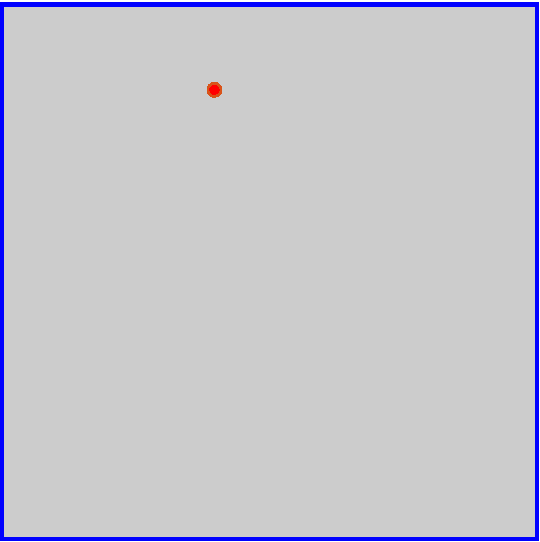
\includegraphics[width=0.25\textwidth]{figures/L21/quadtreeBoxesLevel00-crop.pdf}
    L1: 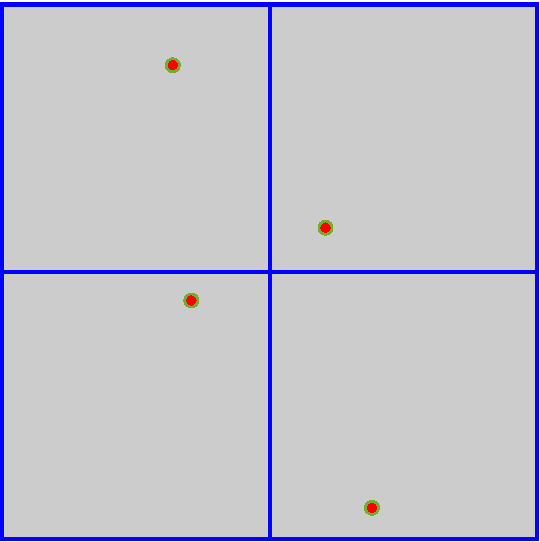
\includegraphics[width=0.25\textwidth]{figures/L21/quadtreeBoxesLevel01-crop.pdf}
    L2: 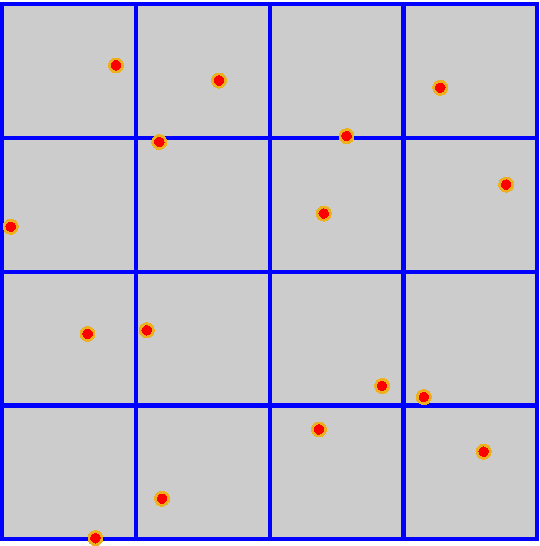
\includegraphics[width=0.25\textwidth]{figures/L21/quadtreeBoxesLevel02-crop.pdf}\\ \vspace{8pt}
    L3: 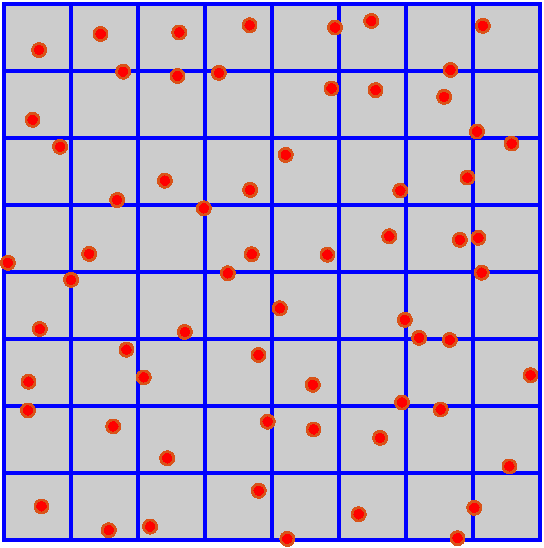
\includegraphics[width=0.25\textwidth]{figures/L21/quadtreeBoxesLevel03-crop.pdf}
    L4: 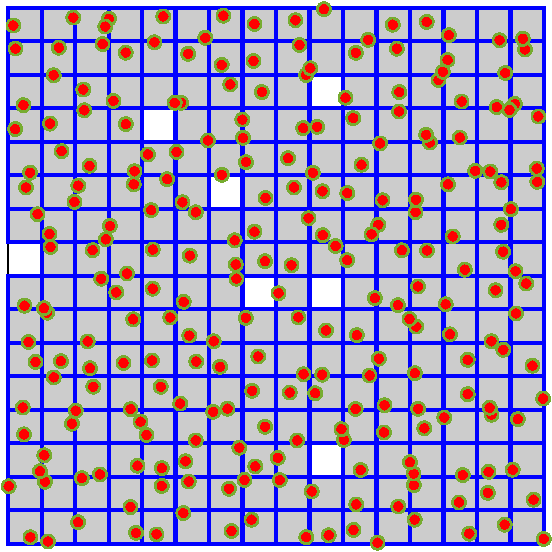
\includegraphics[width=0.25\textwidth]{figures/L21/quadtreeBoxesLevel04-crop.pdf}
    L5: 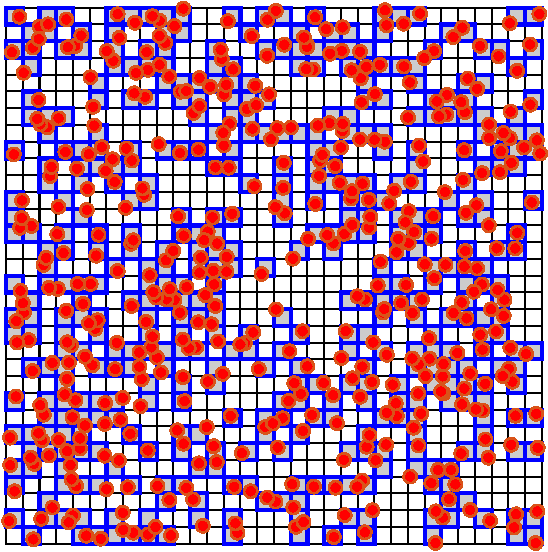
\includegraphics[width=0.25\textwidth]{figures/L21/quadtreeBoxesLevel05-crop.pdf}\\ \vspace{8pt}
    L6: 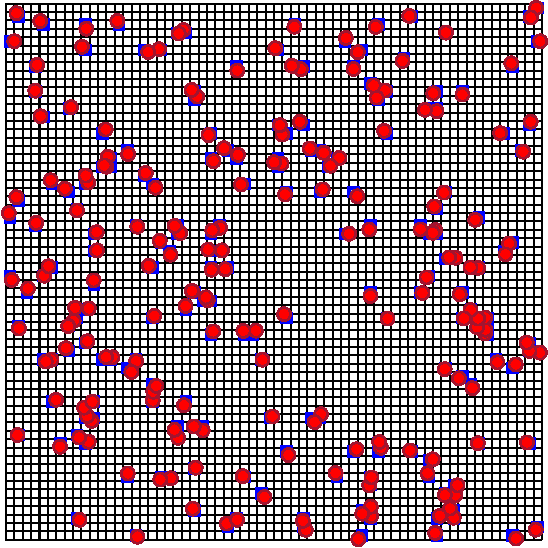
\includegraphics[width=0.25\textwidth]{figures/L21/quadtreeBoxesLevel06-crop.pdf}
    L7: 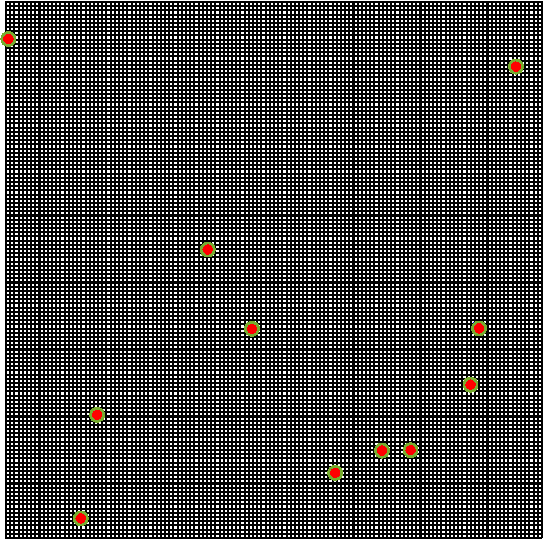
\includegraphics[width=0.25\textwidth]{figures/L21/quadtreeBoxesLevel07-crop.pdf}

    \caption{Eight levels of a quadtree used to store 1024 randomly distributed data points. Notice that each gray box on each level only stores one data point shown as a red circle. }
    \label{quadtreeExample.fig}
\end{figure}


\subsection{Quadtree algorithm cost analysis}

An important remaining question is: what is the cost of inserting $N$ data points into a quadtree ? In the case of uniformly distributed data we can expect with high probability that the insertion time for $N$ data points is $\mathcal{O}(N\log_4(N))$. 

The $\mathcal{O}(.)$ notation is often times referred to as the ``big-O'' notation. In the above notation it implies that asymptotically as $N\rightarrow\infty$ the operational cost is bounded by $CN\log_4(N)$ for some finite constant $C$ that is independent of $N$. 

The estimate pivots on the estimate that for sufficiently well distributed data the cost of inserting point $n$ into a quadtree depends on the depth of the tree. Assuming that the point distribution of the first $n-1$ data points resulted in a tree of depth $\log_4(n-1)$ and observing that the cost of point insertion is proportional to the depth of the tree (number of generations of children boxes) then the total is
\[
\sum_{n=1}^{N} \log_4(n),
\]
which can be bounded with a rough bound as follows
\[
\sum_{n=1}^{N} \log_4(n) \leq \log_4(N) \sum_{n=1}^{N} 1 \leq N\log_4(N). 
\]

In this analysis we assumed that the data points are uniformly distributed and the point insertion process results in a tree structure that is uniformly branching, i.e. almost every box has four children and all levels fill progressively without leaving a large number of empty boxes spread over a large number of levels. The $\log_4$ term results from the assumption that the tree is at most $log_4(N)$ deep. 

In the esoteric case where all points in the data set are the same this analysis is no longer appropriate and the asymptotic cost analysis would degrade to $\mathcal{O}(N^2)$ since inserting point $n$ would involve traversing through the $n-1$ prior inserted boxes. However, this is a relatively pathological limit.

\subsection{Quadtree traversal}

The quadtree data structure can be easily traversed for instance to find data points that are near query points. The simplest way to approach this is to view the process as following the same recursive traversal as the point insertion algorithm, but without inserting the query point in the quadtree. By which we mean we traverse the quadtree starting from the largest box and recursively following the pointer link lists to find a child box that contains the query point but also has no descendent child quadrants. 

We recursively traverse the quadtree with the following function called \texttt{boxPointFindBase}. It checks the child quadrants of a box to see if the query point is included in the child and then recursively calls itself with the child. It keeps doing this until there it finds a box that both includes the query point and has no children. As always the recursive nature of this function makes it a little tricky to discern how it works.
\begin{minted}{c}
box2d *boxPointFindBase(box2d *box, point2d_t *p){

  if(box->childSE)
    if(boxPointInsideSloppy(box->childSE, p, 0))
      return boxPointFindBase(box->childSE, p);

  if(box->childNE)
    if(boxPointInsideSloppy(box->childNE, p, 0))
      return boxPointFindBase(box->childNE, p);

  if(box->childNW)
    if(boxPointInsideSloppy(box->childNW, p, 0))
      return boxPointFindBase(box->childNW, p);

  if(box->childSW)
    if(boxPointInsideSloppy(box->childSW, p, 0))
      return boxPointFindBase(box->childSW, p);

  return box;
}
\end{minted}
This function is called with the largest quadtree \texttt{box} and for each child descendent it uses the \texttt{boxPointInsideSloppy} function to decide if the query point is inside the descendent. If the query point is inside the descendent then the function recursively calls itself and this is process is repeated until the query point is found to be contained inside a box that has no descendent children. 

This function is called in our example code from the \texttt{main} function as follows

\begin{minted}{c}
  point2d_t query;
  query.x = 0.01;
  query.y = 0.6;

  // find box containing q    
  box2d *base = boxPointFindBase(quadtree, &query);
\end{minted}
For a quadtree built with uniformly distributed data points and possessing $\mathcal{O}(\log_4(N))$ levels of recursion the traversal will take $\mathcal{O}(\log_4(N))$ operations. For large $N$ this is significantly faster than performing a brute force search that would take $\mathcal{O}(N)$ to identify nearby points. Furthermore, because the found box must contain both the query point and a point from the data set we know an upper bound on the distance from the query point to the nearest data point which may be contained in a nearby box in the quadtree that does not contain the query point. 

In the next section we describe how to use this information to further find the nearest point in the data set to the query point.

\subsection{Quadtree nearest neighbor algorithm}

In the previous section we presented a construction for a quadtree and described how we can rapidly traverse the data structure to find nearby data points to a query point. In this section we introduce a nearest neighbor algorithm to find the exact nearest neighbor of a query point.

The first step of the nearest neighbor algorithm is to use the recursive \texttt{boxPointFindBase} function described in the previous section to find the smallest box in the quadtree that contains the query point. By construction that box must contain a data point and thus we can compute an upper bound on the distance between the query point and the (as yet unknown) nearest data point. We will call this upper bound \texttt{dMin}. 

The second step again revolves around a recursive traversal of the quadtree. However, this time we traverse the tree looking for boxes that when enlarged by \texttt{dMin} in each direction contain the query point. Starting at the mother box we recursively search each child box that when enlarged by this amount contains the query point. This effectively widens the number of boxes searched so that even boxes that do not contain the query point but may contain the nearest neighbor to that point will be searched for the nearest neighbor.

\begin{minted}{c}
double nearestNeighborSearch(box2d *box, point2d_t *query, point2d_t *nearest){

  double dMin = distanceSquared(query, nearest);
  
  /* check this box first */
  double d = distanceSquared(query, &(box->val));
  if(d<dMin){
    dMin = d;
    *nearest = box->val;
  }

  dMin = sqrt(dMin);

  if(box->childNE)
    if(boxPointInsideSloppy(box->childNE, query, dMin))
      dMin = nearestNeighborSearch(box->childNE, query, nearest);

  if(box->childNW)
    if(boxPointInsideSloppy(box->childNW, query, dMin))
      dMin = nearestNeighborSearch(box->childNW, query, nearest);

  if(box->childSE)
    if(boxPointInsideSloppy(box->childSE, query, dMin))
      dMin = nearestNeighborSearch(box->childSE, query, nearest);

  if(box->childSW)
    if(boxPointInsideSloppy(box->childSW, query, dMin))
      dMin = nearestNeighborSearch(box->childSW, query, nearest);

  return dMin;
}
\end{minted}

{\bf Note}: the \texttt{nearestNeighborSearch} checks the point data contained in each box as it passes through the quadtree as these could be the nearest data points even though they are not at the end of the tree.

\subsection{Quadtree recursive book keeping}

There are some additional functions that we added to help clean up a quadtree that we no longer need (\texttt{boxDestructor}) and to print out a quadtree for visualization in MATLAB (\texttt{boxPrint}).

The destructor follows the same recursive traversal

\begin{minted}{c}
// recursively destruct box         
box2d *boxDestructor(box2d *box){

  if(box->childSE){
    boxDestructor(box->childSE);
    free(box->childSE);
    box->childSE = NULL;
  }

  if(box->childNE){
    boxDestructor(box->childNE);
    free(box->childNE);
    box->childNE = NULL;
  }

  if(box->childSW){
    boxDestructor(box->childSW);
    free(box->childSW);
    box->childSW = NULL;
  }

  if(box->childNW){
    boxDestructor(box->childNW);
    free(box->childNW);
    box->childNW = NULL;
  }
}
\end{minted}

Likewise the quadtree printer recursively prints out the rectangle for each box

\begin{minted}{c}
void boxPrint(FILE *fp, box2d *box, int lev){

  if(box->childSE) boxPrint(fp, box->childSE, lev+1);
  if(box->childNE) boxPrint(fp, box->childNE, lev+1);
  if(box->childSW) boxPrint(fp, box->childSW, lev+1);
  if(box->childNW) boxPrint(fp, box->childNW, lev+1);

  fprintf(fp, "%g,%g,%g,%g,%g,%g,%g\n",
          box->xmin, box->xmax, box->ymin, box->ymax, (double)lev, box->val.x, box->val.y);
}
\end{minted}

\section{Summary}

In this section we have introduced two straightforward concepts. Firstly a quadtree data structure with best case $\mathcal{O}(\log_4(N))$ operational cost to insert a data point or to find a nearest data point. Secondly the construction and queries of the quadtree rely heavily on the use of recursive functions.

\printbibliography[heading=subbibliography]